\documentclass[border=10pt]{standalone}
\usepackage{tikz}
\usetikzlibrary{automata, positioning, arrows}

\begin{document}
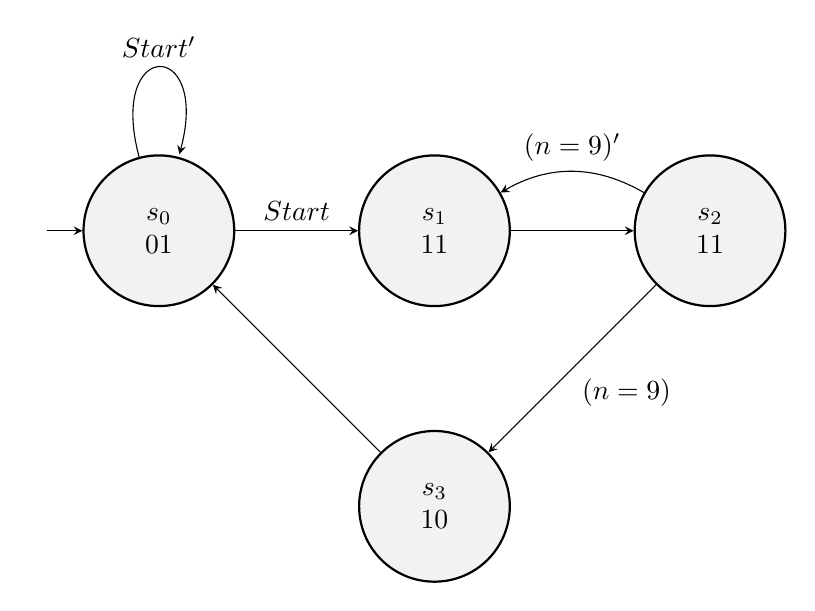
\begin{tikzpicture}[
    ->, >=stealth, auto, node distance=3.5cm,
    every state/.style={thick, fill=gray!10, text width=1.5cm, align=center},
    initial text=$ $
]

    % States with Outputs (Moore)
    % s0/01, s1/11, s2/11, s3/10
    \node[state, initial] (s0) {$s_0$ \\ $01$};
    \node[state, right of=s0] (s1) {$s_1$ \\ $11$};
    \node[state, right of=s1] (s2) {$s_2$ \\ $11$};
    \node[state, below of=s1] (s3) {$s_3$ \\ $10$};

    % Transitions
    \draw   (s0) edge[loop above] node {$Start'$} (s0)
            (s0) edge node {$Start$} (s1)
            (s1) edge node {} (s2)
            (s2) edge[bend right] node[above] {$(n=9)'$} (s1)
            (s2) edge node {$(n=9)$} (s3)
            (s3) edge node {} (s0);

\end{tikzpicture}
\end{document}
